\documentclass{article}
\usepackage{graphicx} % Required for inserting images
\graphicspath{ {images/} }
\usepackage{subcaption} 
\usepackage[catalan]{babel}
\usepackage{amsmath}
\usepackage{amssymb}
\usepackage{color}
\usepackage[style=apa]{biblatex}
\usepackage[a4paper, inner=0.75cm, outer=2cm, top=2.5cm, bottom=2.5cm, bindingoffset=1.2cm]{geometry}
\addbibresource{referencies.bib}  % Link to your .bib file

\begin{document}
\setlength{\parindent}{0pt}

\begin{titlepage}
    \centering
    {\bfseries\LARGE Universitat de Girona \par} \vspace{1cm}
    {\scshape\Large Facultat de Ciències \par}\vfill
    {\scshape\LARGE CARACTERITZANT LA COLONITZACIÓ I EL RISC D'EXTINCIÓ POTENCIAL DE 12 ESP\`ECIES DE PAPALLONES DE CATALUNYA\par} \vspace{2cm}
    % {\Large Treball de Fi Grau \par} \vfill
    % {\scshape\Large Facultat de Ciències \par}\vfill
    % {\scshape\LARGE CARACTERITZANT LA DISPERSIÓ I EL RISC D'EXTINCIÓ POTENCIAL DE LES POBLACIONS DE PAPALLONES DE CATALUNYA\par} \vspace{2cm}
    % {\Large Treball de Fi Grau \par} \vfill

    {\large \textbf{Autor:} Joana Violeta Dekker \par}\vspace{0.1cm}
    {\large \textbf{Grau:} Ci\`encies ambientals \par}\vspace{0.1cm}
    {\large \textbf{Centre:} CEAB-CSIC \par}\vspace{0.1cm}
    {\large \textbf{Tutors: } David Alonso i Vicente J. Ontiveros\par}\vspace{0.1cm}
    {\large \textbf{Estada: } 1 de Juliol a 11 de Setembre \par}\vspace{1cm}
    {\large \textbf{} 12 de Setembre de 2024 \par}
\end{titlepage}

\newpage
\tableofcontents
\newpage
\section{Introducció}

Durant les darreres dècades, la intensificació de l'activitat humana ha sovint resultat en la deterioració dels ecosistemes, la pèrdua de biodiversitat i la disseminació d'espècies no aut\`octones, entre altres efectes (\cite{gotelli_2008}). Una estratègia eficaç per avaluar la conservació dels sistemes naturals i implementar mesures de protecció és el monitoratge d'espècies bioindicadores. Aquest tipus de monitoratge consisteix a realitzar censos repetits i periòdics al llarg de transectes constants, amb l'objectiu de recopilar dades sobre la pres\`encia i  l'abundància d'un organisme (o grup d'organismes) al llarg del temps, permetent així avaluar les variacions poblacionals a la regió en estudi.
\smallskip

Segons el tipus d'impacte i l'entorn que es pret\'en analitzar, com poden ser la contaminació del sòl, de l'aire, la qualitat de l'aigua o la disponibilitat d'aliments, es pot seleccionar el grup de bioindicadors més adequat. Aquest grup ha de complir amb certs criteris: mostrar alta sensibilitat i reaccionar amb rapidesa als canvis ambientals, ser fàcilment reconeixible i incloure diverses espècies que abastin un ampli rang d'hàbitats diferents. Les papallones satisfan tots aquests criteris.
\smallskip

Les papallones diürnes (ropalòcers), juntament amb les arnes (heteròcers), formen l'ordre dels lepidòpters. En total, existeixen aproximadament 160.000 espècies a nivell mundial (\cite{lepidopters2023}). Els ropalòcers són reconeguts com a valuosos indicadors ambientals (\cite{thomas2005}) per diverses raons: tenen un cicle de vida curt, una limitada capacitat de dispersió, depenen d'unes poques plantes nutricies, són fàcils d'identificar i són populars entre el públic en general. Per aquestes raons, molts països han implementat programes de seguiment a llarg termini. El Regne Unit va ser el primer país a establir un sistema estandarditzat per al monitoratge amb el United Kingdom Butterfly Monitoring Scheme (UKBSM) durant la dècada dels 1970. Gradualment, altres països van començar a adoptar aquest sistema. A Catalunya, l'any 1994 es van establir els primers punts de monitoratge del Catalan Butterfly Monitoring Scheme (CBMS), un projecte coordinat des del Museu de Ci\`encies Naturals de Granollers, una xarxa que s'ha anat ampliant per tota la geografica catalana i les illes Balears fins a comptar a amb 254 punts de mostreig el 2024. Finalment, ja el 2004 es va fundar la Butterfly Conservation Europe, amb l'objectiu de coordinar els esforços de monitoratge dels diversos pa\"isos europeus.
\smallskip

En aquest treball ens proposem estudiar la din\`amica de colonitzaci\'o i extinci\'o de 12 esp\`ecies de papallones diurnes en el conjunt dels transectes que conformen el CBMS. Proposarem una nova caracterizaci\'o de cada esp\`ecia. Com expliquem m\'es endavant, utilitzarem un model que t\'e els seu inicis en la teoria de biogeografia d'illes de MacArthur i Wilson (\citeyear{MacArthurWilson67}), on cada esp\`ecie, de forma molt simple, queda definida per nom\'es un parell de par\`ametres: la seva taxa d'extinci\'o i la seva taxa de (re-)colonitzaci\'o. Un dels objectius principals d'aquest treball és comparar com la caracterització que proposem es relaciona amb altres caracteritzacions prèviament establertes per altres investigadors. 
\smallskip

Anteriorment, investigadors del CBMS van introduir dos indexos per caracteritzar el grau d'especialitzaci\'o de les esp\`ecies de papallones de Catalunya (\cite{stefanescu2011-SSI,colom2022-HPI}) (veure tab \ref{tab:species_indices}), i tamb\'e van estimar la seva capacitat de dispersió o mobilitat. En aquest treball estudiarem nom\'es 12 esp\`ecies (veure tab \ref{tab:species_indices}). L'elecci\'o en concret d'aquestes esp\`ecies permet considerar un ventall ampli de possibilitats (des d'esp\`ecies molt generalistes, a molt especialitzades, i des d'esp\`ecies migradores a esp\`ecies poc m\`obils).  L'índex SSI (Specialisation Score Index) mesura la preferència d'hàbitats d'una esp\`ecie a partir de la fracci\'o d'habitat que ocupa aquesta en relaci\'o al nombre d'habitats possibles (\cite{julliard2006-SSI}). Aquest índex quantifica el grau d'especialització d'una espècie respecte als diferents hàbitats, assignant valors més alts a les espècies especialistes i més baixos a les generalistes. L’HPI (Host-Plant Index) mesura quantes espècies de plantes nutrícies pot utilitzar una papallona per al desenvolupament larvari (\cite{Middleton-WellingJoseph2020-HPI}). Segons el nombre i diversitat de plantes hoste que una espècie pot aprofitar, s’assigna un valor d’índex que indica si l'especies es \textit{especialista} (valor alt), \'es a dir, utilitza molt poques espècies de plantes, sovint d’un sol gènere o família, o b\'e \textit{generalista} (valor baix), \'es a dir, pot utilitzar moltes espècies de plantes d’una àmplia varietat de famílies. 
 
\section{Metodologia}
\subsection{Els indexos}
Una manera d'ordenar les espècies és segons el grau d'especialització. Teòricament, l'especialització d'una espècie es calcula segons l'amplitud del nínxol ecològic considerant totes les dimensions (llegir apunts d'ecologia). A la pràctica, s'ha anat proposant i utilitzant mètodes propis i més idonis per cada grup d'espècies segons les característiques particulars de cadascun dels grups. 


\subsubsection{SSI}
Una forma més general de quantificar l'especialització és comptant els diferents hàbitats en què es coneix que l'espècie és present. Aquesta mesura permet ordenar les espècies en un gradient de menys especialista (present en un nombre menor d'hàbitats diferents) a més generalista (present en un nombre major d'hàbitats diferents). Tanmateix, aquesta aproximació ignora les possibles grans variacions de densitat de les diferents categories d'hàbitat. De tal manera que dues espècies es considerarien igual de generalistes — segons les dades de presència-absència— ignorant la densitat en què aquestes espècies es troben en els hàbitats. Per tant, per tenir en compte la variació de densitat entre hàbitat, es quantifica el grau d'especialització d'hàbitat com la variància de densitats mitjanes entre les 20 categories d'hàbitat considerades (citar cbms, o una taula amb els). Per obtenir una mètrica estadísticament independent de la densitat mitjana de les espècies, el que es fa és utilitzar el coeficient de variació (desviació estàndard/mitjana) com a mesura de cada índex d'especialització de les espècies (SSI).

\subsubsection{HPI}
Una aproximació més pròpia per a l'estudi del grau d'especialització de les espècies de papallones és el Host Plant Index (HPI) (Warren et al. 2001)


\subsubsection{Mobilitat}
<breu descripci\'o>

\subsection{Les dades: transectes BMS}
El n\'umero de transectes del CBMS han anant augmentant al llarg dels anys (veure gr\`afica \ref{fig:IDsPerAny}). Tot i que els transectes no estan distruits per tot Catalunya i Balears de forma homog\`enia, cobreixen tres regions bioclim\`actiques diferenciades: l'\`area alpina i subalpina, l'\`area mediterr\`nia humida (def???) i l'\`area mediterrani \`arida (def???). 

\begin{figure}
  \centering
  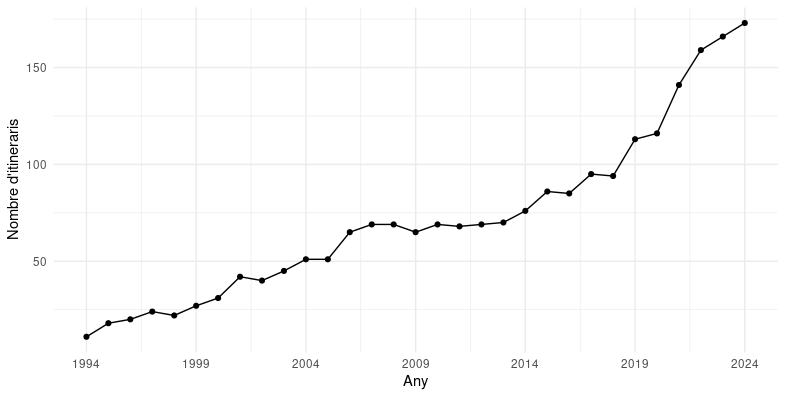
\includegraphics[scale=0.8]{nombre-itineraris-per-any.png}
  \caption{\label{fig:IDsPerAny} \textbf{Nombre d'itineraris actius per any del CBMS}.}
\end{figure}
 
\smallskip

% (Teoria biogeografica d'illes -> model dinamic c-e)

 
\subsection{Les espècies}
Les esp\`ecies que hem estudiat s\'on les seg\"uents: 

\begin{enumerate}
    \item {\it Pseudophilotes panoptes} (Hübner, 1813)- Blaveta de la farigola (cat): Univoltina primaveral, generalment vola des de març a maig, amb un pic a l'abril, tot i que se l'ha vist volar a Puerto de La Ragua, Granada fins a finals de juny. Planta nutrícia: diverses espècies de Timó (Thymus spp.). Habitat: 0 - 1000 m. Sovint es troba en zones àrides, amb presència de Timó. Identificació: El mascle és de color blau cel metal·litzat i la femella marró. Presenten unes fímbries blanques i negres al marge. Aquesta espècie de papallona és coneguda per les seves ales de color blau amb taques negres i taronges en el seu marge exterior. Habitat: Sovint es troba en zones àrides, amb presència de Timó. 
    
    \item {\it Lycaena virgaureae} (Linneaus, 1758) - Coure roent (cat): Univoltina, en vol des de finals de juny fins finals de setembre. Planta nutrícia: Agrella (R. acetosa) i agrelleta o sang de Jesucrist (R. acetosella). Identificació: Mascle amb l'anvers d'un intens color taronja llis i un marge negre, i la femella amb diverses taques negres sobre fons taronja i el marge negre més marcat. Habitat: 500 - 2.200 m. Freqüent en prats, també en pinars. 
    
    \item {\it Plebejus argus} (Linnaeus, 1758) - Blavet argiu (cat): A la península, univoltina, a Catalunya s'han observat fins a tres generacions, amb un període de vol des de finals d'abril fins a octubre. Planta nutrícia: gran varietat d'espècies, des dels Trifolium, Ulex, Astragulus, Colutea, Genista, Coronilla i Caluna spp. Identificació: Marcat dimorfisme sexual, amb el mascle de color blau marí metàl·lic i una ampla banda marginal negre, i la femella marró. El revers presenta una banda taronja submarginal i una blanquinosa postdiscal. Habitat: 0 - 2.400 m. Es troba preferentment en zones humides de muntanya però també en prats, matollars, clarianes de muntanya i barrancs muntanyencs.
    
    \item {\it Cyaniris semiargus} (Denis and Schiffermuller, 1775) - Cobalt (cat): Univoltina, en vol des de mitjans de maig fins principis d'agost. Planta nutrícia: trèvol comú (Trifolium pratense), trevolet (T. repens), armeria (Armeria maritima) i A. alliasea. Identificació: Marcat dimorfisme sexual; amb l'anvers del mascle de color blau cobalt i la femella marró. Revers gris marronós, amb escates blavoses a la base de l'ala posterior, i una sèrie de punts negres encerclats de blanc a les ales anterior i posterior. Habitat: 500 - 2.400 m. Freqüenta àrees ruderals, prats montans, conreus i zones humides de muntanya.
    
    \item {\it Vanessa cardui} (Linnaeus, 1758) - Migradora dels cards (cat): Polivoltina i migradora. Planta nutrícia: gran varietat de plantes, especialment cards (Cirsium i Carduus spp.). Identificació: Anvers amb fons ataronjat amb taques negres, i les puntes negres amb taques blanques. Al revers de les ales posteriors hi destaquen 4 i 5 ocels blau-negres. Habitat: 0 - 3000 m. Es troba en tots els ambients que hi hagi nèctar, en gairebé tots els continents del món.

    
    \item {\it Celastrina argiolus} (Linnaeus, 1758) - Blaveta de l'heura (cat): Polivoltina, possiblement amb una quarta generació parcial en moltes localitats. En vol des de finals març fins a finals de setembre. Planta nutrícia: gran varietat d'espècies; com heures (Hedera), (Genista), (Rubus) i (Ilex). Identificació: Coloració blava pàl·lida amb puntets negres allargats a les ales anteriors i arrodonits a les posteriors. També és força generalista, colonitza jardins, prats, matollars, zones arbrades zones humides i conreus, entre altres.
    
    \item {\it Aglais io}(Linnaeus, 1758) - Paó de dia (cat): Polivoltina, en vol des de febrer fins a finals d'agost. Planta nutrícia: Ortiga comuna (Urticaria dioica) i ocasionalment el llúpol (Humulus lupulus). Identificació: Les seves ales presenten una coloració marró rogenca amb una gran taca a l'anvers de l'ala posterior semblant a un ull de color blau i negre. El revers és de color fosc. Habitat: 0 - 2500 m. És comú en un bon nombre d'habitats (zones humides de muntanya, prats, boscos, conreus, parcs i jardins, i zones revegetades). 
    
    \item {\it Pyronia cecilia}(Vallantin, 1894) - Saltabardisses de solell (cat): Univoltina, en vol des de finals d'abril fins a l'agost. Planta nutrícia: Llistó (Brachypodium retusum) i fenàs de marge (B. phoenicoides). Identificació: Anvers ataronjat amb grans marges obscurs. Presenta un ocel negre amb dos nuclis blancs a l'ala anterior. Al revers de l'ala posterior és gris jaspiat sense ocels. Habitat: 0 - 1200 m. Prefereix les regions càlides i assolellades del sud d'Europa, com prats mediterranis, parcs, matollars, boscos esclerofil·les conreus, fruiterars i platges.
    
    \item {\it Melanargia occitanica} (Esper, 1793) - Escac ferruginós (cat): Univoltina, en vol des d'abril fins a mitjans de juny. Planta nutrícia: fenàs de marge (Brachypodium phoenicoides), llistó (B. retusum), llambra (Stripa offneri), S. lagascae) i l'espart bord (Ligerum spartum). Identificació: L'anvers és de color blanc amb abundants taques negres i fímbries escaquejades. Habitat: 0 - 1500 m.  Prats, matollars, conreus, zones sense vegetació i parcs.

    \item {\it Pararge aegeria} (Linnaeus, 1758) - Bruna del bosc (cat): Polivoltina, en vol des de marc a octubre. Planta nutrícia: fenàs de bosc (Branchypodium sylvaticum), dàctil (Dactylis glomerata), l'agram prim (Elymus repens), el ripoll (Oryzopsis miliacea), entre moltes altres. Identificació: Caracteritzada per un dibuix de color marró amb taques ataronjades. Habitat: 0 - 1200 m. Es troba comunament en boscos més aviat humits i densos, de ribera, zones humides, matollars alts, parcs i jardins.

    \item {\it Pyronia bathseba} (Fabricus, 1793) - Saltabardisses cintada (cat): Univoltina, en vol des de finals d'abril fins finals de juliol. Planta nutrícia: herbes, en especial Branchypodium phoenicoides i probablement B. retusum, com també la poa comú (Poa trivialis). Identificació: Ales amb taques arrodonides amb un ressaltat taronja i una característica cinta blanca. Habitat: 0 - 1200 m. Sovinteja ecosistemes càlids, amb boscos oberts, matollars, prats, conreus i zones urbanitzades


    \item {\it Anthocharis euphenoides} (Staudinger, 1869) - Aurora groga (cat): Univoltina primaveral, en vol des de març fins a juny (o juliol al Pirineu). Planta nutrícia: Principalment, plantes del gènere Biscutella spp, però també Sisymbrium, Sinapis i Capsella spp.  Identificació: Marcat dimorfisme sexual; el mascle amb coloració groguenca a l'anvers i una taca taronja vermellosa situada a la meitat externa de l'ala anterior, i la femella és blanca amb la taca d'un ataronjat més grisós. Habitat: 0 - 1.800 m. Es pot trobar en un bon nombre d'habitats, des de boscos, matollars, prats, conreus i zones sense vegetació.
\end{enumerate}

\begin{table}[h]
  \centering
  \begin{tabular}{|c|c|c|c|c|}
    \hline
    Espècie & Categoria UICN &SSI Index & HPI Index  & Mobilitat\\ \hline
    \textit{Pseudophilotes panoptes} & \color{red}{LC} & Alt (1.430) & Alt (0.577) & \textit{1}\\ \hline
    \textit{Lycaena virgaureae} & LC & Alt (2.552) & Alt  (0.707) & \textit{2}\\ \hline
    \textit{Plebejus argus} &  LC & Alt (2.403) & Baix (0.129) & \textit{1}\\ \hline
    \textit{Cyaniris semiargus} & LC & Alt (2.263) & Baix (0.183) & \textit{1}\\ \hline
    \textit{Vanessa cardui} & LC & Baix (0.813) & Baix (0.019) & \textit{4}\\ \hline
    \textit{Celastrina argiolus} & LC & Baix (0.593) & Baix (0.044)& \textit{3}\\ \hline
    \textit{Aglais io} & LC & Baix (0.831) & Alt (0.544) & \textit{3}\\ \hline
    \textit{Melanargia occitanica} & NT & Alt (1.314) & Mig (0.354) & \textit{2}\\ \hline
    \textit{Pararge aegeria} & LC & Mig (0.942) & Baix (0.111) & \textit{3}\\ \hline
    \textit{Pyronia cecilia} & LC & Baix (0.796) & Alt (0.707) & \textit{2}\\ \hline
    \textit{Pyronia bathseba} & LC & Baix (0.764) & Mig (0.408) & \textit{2}\\ \hline
    \textit{Anthocharis euphenoides} & LC & \color{red}{Mig (0.652)} & Alt (0.667) & \textit{2}\\ \hline
  \end{tabular}
  \caption{Taula de les esp\`ecies de papallones estudiades amb en les categories UICN, LC correspon a preocupacio menor (least concern), i NT gairabé amenaçada (near threatened). Els índexos SSI, HPI, i mobilitat o capacitat de dispersi\'o.(\cite{ubach2025})}
  \label{tab:species_indices}
\end{table}

\subsection{El model}
El model utilitzat s'inspira en la teoria de biogeografia d'illes (\cite{MacArthurWilson67}). Aquesta teoria incialment va ser proposada per entendre la davallada que s'observa en el nombre d'esp\`ecies d'una comunitat determinda en un conjunt d'illes cada cop m\'es allunyades d'un contitent. Encara que no s'esmenta habitualment, aquesta teoria fa dues hip\`otesis essencials. Per una banda, cal assumir que les esp\`ecies tenen din\`amiques independents ({\it hip\`otesi d'independ\`encia}), \'es a dir, per construir el model cal considerar que la pres\`encia de cap esp\`ecie no influeix en la probabilitat d'extinci\'o de cap esp\`ecie present o en la probabilitat de colonitzaci\'o de cap esp\`ecie que potentialment podria arribar al territori en q\"uesti\'o. Per una altre, cal tamb\'e assumir que les esp\`ecies de la communitat s\'on prou similars com per considerar que les probabilitats d'extinci\'o i colonitzaci\'o no depeden, si fa no fa, de la identitat de cada espe\`ecie ({\it hip\`otesi d'equival\`encia}). Per tant, la teoria es basa en aquestes dues hip\`otesis fonamentals: independ\`encia i equival\`encia. Metre que la primera hip\`otesi \'es complicat de relaxar ja que necessitar\'iem tenir alguna idea de com interaccionen aquestes esp\`ecies entre s\'i (si s\'on o no fortes competidores o mutulistes i fins a quin punt ho s\'on), en aquest treball, veurem que \'es trivial relaxar la segona hip\`otesi, la qual cosa ens permetr\`a caracteritzar cada esp\`ecie independentmet \'unicament per dos parametres: una taxa de colonitzacion, $c$, i una taxa d'extinci\'o, $e$. 

\subsubsection{La teor\'ia de biogeografia d'illes i de metapoblacions}
Per simplificar, imaginem primer que tenim una esp\`ecie en un continent que alimenta un sistemes d'illes situat a una dist\`ancia determinada del continent. Assumim tamb\'e per simplicar que les illes son prous similars (en \`area, en tipus d'habitat, etc) com per considerar que la probabilitat de persist\`encia (o probabilitat d'extinci\'o) de l'especie en cada illa \'es aproximadament la mateixa. Assumim, a m\'es a m\'es, que totes les illes es troben situades a una mateixa dist\`ancia del continent i, per tant, la probaibitat d'arribada (o colonitzaci\'o) de l'esp\`ecie a cada illa \'es la mateixa. En aquesta situaci\'o podem definir la probabilitat de pres\`encia de l'esp\`ecie en una illa determinada en un moment determinat pel seg\"uent quocient: 
\begin{equation}
    p = \frac{n}{N}
    \label{eq:ocupancia}
\end{equation}
on $n$ \'es el nombre d'illes ocupades per l'esp\`ecie en q\"uesti\'o en un moment determinat i $N$ \'es el nombre total d'illes. Aquesta probabilitat (proporci\'o d'illes ocupades) s'anomena ocup\`ancia observada de l'esp\`ecie en el conjunt de les illes. 
\smallskip

A tall d'exemple, l'ocup\`ancia de cada esp\`ecie de papallona evoluciona en el temps. Usant l'Eq (\ref{eq:ocupancia}), la podem calcular si considerem que els transectes ($N$) del CBMS s\'on prou similars, i simplement en comptem en quants hi apareix una esp\`ecies en q\"uesti\'o durant un conjunt d'anys successius (la $n$ a l'equaci\'o anterior), com es pot veure a la figura (veure figura). Si totes els transectes s\'on prou similars (en llurs condicions ambientals), la probabilitat de pres\`encia d'aquesta esp\`ecie en cadascun d'ells seria la mateixa i coincidiria amb aquesta occup\`ancia calculada. A la pr\`actica, com demostrarem, aquesta tercera hip\`otesi addicional {\it d'homogene\"itat ambiental} no es compleix, i aquesta ocup\`ancia calculada \'es simplement una occup\`ancia mitjana de l'esp\`ecie en questi\'o al conjunt del CBMS. L'evoluci\'o temporal de les occup\`ancia d\'ona idea de si una esp\`ecie est\`a en regressi\'o o expansi\'o geogr\`afica. 
\smallskip

Hem vist que l'ocup\`ancia observada o emp\'irica de cada esp\`ecie de papallona evoluciona en el temps (veure figura).  Si admetem que hi ha homegene\"itat ambiental, com podr\'iem calcular te\`oricament l'evoluci\'o temporal de l'ocup\`ancia d'una esp\`ecie en el conjunt de les $N$ localitats considerades? 
\smallskip

La pregunta anterior est\`a a cavall entre dos grans marcs conceptuals de la ci\`encia ecol\`ogica, la teoria de biogeografia d'illes i la de metapoblacions (\cite{gotelli_2008}). Si ens centrem en una sola esp\`ecie, les $N$ localitats (o itineraris) considerades constituirien una metapoblaci\'o. Si considerem un conjunt d'esp\`ecies equivalents, $S_M$, amb din\`amiques independents, llavors el producte $S_M$, per l'ocup\`ancia $p$ representa el numero mitj\`a d'esp\`ecies que s'espera trobar en un d'aquestes localitats, i la pregunta anterior \'es precisament la que es van fer MacArthur i Wilson (\citeyear{MacArthurWilson67}) quan van presentar la seva teoria. 
\smallskip

En qualsevol cas, dos processos elementals governen la pres\`encia d'una especies en una localitat determinada: 

\begin{enumerate}
\item \textbf{Colonitzaci\'o} Una esp\`ecie pot colonitzar una localitat (representada per cada cada itinerari o transecte mostrejat) a un taxa $c$. Aquest proces \'es inherentment estocastic. Si en un total de $N$ localitats, $n$ presenten l'esp\`ecie en q\"uesti\'o (i, per tant, $n_0 = N-n$, no que l'hi preseten), $c\, n_0$ seria el nombre de localitats colonitzades per l'esp\`ecie en q\"uesti\'o per unitat de temps (de les $n_0$ localitats on no hi trobem l'esp\`ecie analitzada). Quines d'aquestes patitirien aquestes colonitzacions \'es un proc\'es totalment aleatori. 

\item \textbf{Extinci\'o} L'esp\`ecie pot desapar\`eixer d'una localitat determinada a una taxa $e$. En el conjunt de les $n$ localitats on si que hi \'es l'esp\`ecie analitzada, el producte $e\,n$ seria el nombre de localitats que enregistrarien l'extinci\'o de l'esp\`ecie en q\"uesti\'o per unitat de temps, per\`o quines localitats concretes realment patirien aquestes extincions seria de nou totalment aleatori.
\end{enumerate}
\smallskip

\'Es important remarcar que el model que presentem fa \'us de dos constructes te\`orics: el continent (o la metacommunitat) i un cojunt de $N$ localitats equivalents. El primer es la font de la qual provenen les esp\`ecies  que colonitzen de forma independent la localitat en q\"uesti\'o, per\`o no existeix en realtitat. De fet, assumirem impl\'icitament que les esp\`ecies provenen {\it de tot arreu}. Models metapoblacionals realistes (\cite{hanski1991single,hanski2004ecology}) que considerin la dispersi\'o entre localitats tot tenint en compte la posici\'o geogr\`afica expl\'icita de cada localitat, per b\'e que ben interessants, queden m\'es enll\`a dels objectius que ens proposem assolir en aquest treball. El segon \'es simplement un constructe matem\`atic que ens permet definir correctament la probabilitat o ocup\`ancia d'una esp\`ecie en una localitat determinada amb unes carecter\'istiques ambientals concretes (com si les $N$ localitats equivalents existissin en realitat). Per exemple, si $n(t)$ \'es el numero de localitats on l'esp\`ecie en q\"uesti\'o \'es present en cert moment $t$, llavors aquest nombre evoluciona en el temps segons l'equaci\'o seg\"uent: 
\begin{equation}
    \frac{dn(t)}{dt} = c\,(N-n(t)) - e\,n(t)
\end{equation}
on $N$ el el nombre de localitats equivalents de qu\`e parl\`avem. Ara podem expressar aquesta equaci\'o en termes de l'ocup\`ancia, si utilitzem la definicio en l'Eq (\ref{eq:ocupancia}), i dividim, membre a membre, l'equacion anterior per $N$:
\begin{equation}
    \frac{dp(t)}{dt} = c\,(1-p(t)) - e\,p(t)
    \label{eq:fonamental}
\end{equation}

Aquesta darrera equaci\'o ser\`a la nostra equaci\'o de partida. En principi, les esp\`ecies poden diferir en llurs taxes de colonitzaci\'o i extinci\'o. Si les esp\`ecies tenen din\`amiques independents, l'evoluci\'o temporal de cadascuna de llurs ocup\`ancies vindr\`a descrita per aquesta mateixa equaci\'o fonamental. Aix\`o significa que el parell $(c_{i},e_{i})$ defineix completament l'espe\`ecie $i$ en un conjunt de localitats amb condicions ambientals equivalents. La teoria de MacArthur and Wilson (\citeyear{MacArthurWilson67}) considera un conjunt d'esp\`ecies equivalents, totes elles descrites pel mateix parell $(c, e)$, on la din\`amica de totes elles segueix la nostra equaci\'o fonamental, Eq. (\ref{eq:fonamental}). Aquest treball se centra en determinar els par\`ametres de colonitzaci\'o i extinci\'o de cada esp\`ecies per separat tot relaxant aix\'i la hip\`otesi d'equival\`encia (tant pel que a les esp\`ecies com pel que fa a les localitats). Per tant, en aquest treball mostrem que una esp\`ecie de papallona pot tenir un parell colonitzaci\'o-exinci\'o que la caracteritza en un conjunt de localitats tipiques d'un cert amibent determinant, per exemple, la muntanya mitjana, i un de different per un conjunt de localitats t\'ipiques d'un altre ambient, per exemple, la terra baixa i humida mediterr\`ania.  
\smallskip

\subsection{An\`alisi de dades: el concepte de m\`axima versemblan\c{c}a} 
Com estimar els par\`ametres d'extinci\'o i colonitzaci\'o de cada esp\`ecie? De entrada, cal dir que el CBMS ens forneix d'un conjunt de dades de gran valor amb un gran nivell de detall. No obstant, l'an\`alisi que presentem aqu\'i en basa en la contrucci\'o de taules agregades de pres\`encies annuals per cada esp\`ecie en q\"uesti\'o. Per tant, la taula de dades de partida representar\`a les pres\`encies annuals d'una esp\`ecie concreta en un conjunt de localitats (transectes o itineraris) a llarg d'una colla d'anys on ha estat mostrejada (Taula \ref{tab:observacions}).   

\begin{table}
    \centering
    \begin{tabular}{l|c|c|c|c}
         ID      & 1995 & 1997 & 2001 & 2005 \\
         \hline
         1       &  0   &   1  &   1  & 0  \\
         $\dots$ & $\dots$ & $\dots$  & $\dots$ & \dots \\  
         23      &  0   &   1  &   0  & 1      \\
         \hline
         n       &  1   &   22 &   21 &  10     
    \end{tabular}
    \caption{Observacions annuals d'una esp\`ecie en un conjunt d'itineraris. La darrara fila representa el nombre d'itineraris en els quals s'ha observat l'esp\`ecie donada a llarg dels anys.}
    \label{tab:observacions}
\end{table}

Com a exemple, imaginem ara que volem estimar els parametres de colonitzacio i extinci\'o d'una esp\`ecie nom\'es a l'itinerari 1. Segons indica la taula \ref{tab:observacions} a la primera fila \ref{tab:observacions}, l'esp\`ecie va ser observada els anys 1997 i 2001, mentre que els anys 1995 i 2005 l'itinerari va ser mostrejat per\`o l'esp\`ecie no va ser observada. Per simplificar, assumirem {\it detectabilitat perfecta}, \'es a dir, si l'esp\`ecie no va ser vista llavors realment no hi era en aquella localitat. En models com el nostre, de colonitzaci\'o i extinci\'o, la hip\`otesi de detectabilitat perfecta es pot relaxar \cite{MacKenzie03}, per\`o cal disposar d'un mostreig amb replicaci\'o, cosa que no sempre \'es possible amb les dades dels transectes CBMS. Necessitar\'iem itineraris amb seccions que es puguin considerar totalment equivalents.
\smallskip

En el desenvolupament que condueix a la construcci\'o de la funci\'o de versemblan\c{c}a que expliquem a continuaci\'o \'es molt important interpretar l'ocup\`ancia introdu\"ida anteriorment (veure Eq. \ref{eq:ocupancia}) com la probabilitat que l'esp\`ecie en q\"uesti\'o estigui present en un itinerari concret en un any determinat. Introduim ara una notaci\'o que explicita aquesta interpretaci\'o i rescrivim la nostra equaci\'o fonamental (veure Eq. \ref{eq:fonamental}) de forma equivalent com: 
\begin{equation}
  \frac{dP(1;t)}{dt}=-e\, P(1,t)+c(1-P(1,t))
  \label{eq:fonamental_Bis}
\end{equation}
on $P(1;t)$ \'es la probabilitat de pres\`encia l'esp\`ecie a l'itinerari l'any $t$, metre que $P(0;t)$ seria la probabilitat d'abs\`encia. Sota la hip\`otesi de detectabilitat perfecta, els 0 i 1 a la taula de dades correponden a abs\`encies i pres\`encies reals, respectivament. 
\smallskip

Pel m\`etode de variaci\'o de constants, l'equaci\'o anterior es pot resoldre: 
\begin{eqnarray}
  P(1;t) & = & \frac{c}{e+c}+C\,\exp(-(e+c)t)\\
  P(1;0) & = & p_{0}\nonumber 
\end{eqnarray}
on $p_0$ representa la condici\'o inicial, \'es a dir, la probabilitat que l'esp\`ecie estigui present al temps inicial, considerat aqui com $t=0$. Per exemple, si $p_0 = 0$, la constant $C$ es pot determinar, la qual cosa condueix a la seguent expressi\'o: 
\begin{equation}
  P(1;t)=\frac{c}{e+c}(1-\exp(-(e+c)t))\label{t_10}
  \label{eq:P1t}
\end{equation}
que ens d\'ona la probabilitat que una esp\`ecie estigui present en una localitat al cap de certs anys $t$ si a l'inici n'era absent. Fixem-nos que la variable $t$ representa {\it l'interval de temps} o els anys trascorreguts entre les dues observacions. De la mateixa manera podem construir la probabitat que l'esp\`ecia hagi desaparegut de l'intenari al cap de cert temps quan a l'inici hi era present, i de fet, les quatre transicions rellevants seg\"uents: 
\begin{equation}
  \label{T_00}
  \left\{
    \begin{array}{ccc}      
      T_{00} &=&  1 - \frac{c}{e+c} ( 1 - \exp(-(e+c)\Delta t))\\
      
      T_{10} &=&  \frac{c}{e+c} ( 1 - \exp(-(e+c)\Delta t) )\\  
      
      T_{01} &=&  \frac{e}{e+c} ( 1 - \exp(-(e+c)\Delta t) ) \\
      
      T_{11} &=&  1 - \frac{e}{e+c} ( 1 - \exp(-(e+c)\Delta t)) 
    \end{array}
  \right.
  \label{eq:matriu}
\end{equation}
on $T_{00}$, $T_{10}$, $T_{01}$, i $T_{11}$ son probabilitats de transici\'o. Les dues primeres reprenten, respectivament, les probabilitats de continuar, a la localitat, sense l'espec\`cie en q\"uesti\'o ($T_{00}$) o observar-ne la colonitzaci\'o ($T_{10}$) al cap de certs anys $\Delta t$ si a l'inici de l'interval l'esp\`ecie no hi era (per aix\`o sumen 1). Les dues darreres representen la probabilitat d'extincti\'o ($T_{01}$) o de continuar observant, a la localitat, l'esp\`ecie en qu\"uesti\'o ($T_{11}$) al cap de certs anys $\Delta t$ si a l'inici de l'interval l'esp\`ecie hi era (per aixo tamb\'e sumen 1). Les 4 probabilitats defineixen un matriu de transicions que inclou els 4 elements possibles. L'eq. (\ref{eq:P1t}) seria l'element $T_{10}$ de la matriu de transicions. 
\smallskip

Ara, bo i admetent detectabilitat perfecta, estem ja en condicions de respondre la pregunta seg\"uent. Donades unes taxes annuals de colonitzaci\'o i extinci\'o, $(c,\,e)$, quina \'es la probabilitat d'haver fet les seg\"uents observacions a l'itineari 1 des del 1995 al 2015? 

\begin{center}
    \centering
    \begin{tabular}{l|c|c|c|c}
         ID      & 1995 & 1997 & 2001 & 2005 \\
         \hline
         1       &  0   &   1  &   1  &   0     \\
         \hline
         $\Delta t$ & - & 2 & 4 & 4   
    \end{tabular}
\end{center}
on $\Delta t$ represnta l'interval temporal entre observacions. 
\smallskip

Utilitzant les expressions de les transicions (Eq. \ref{eq:matriu}), podem escriure aquesta probabilitat com un producte de 3 transcions elementals (o probabilitats de transici\'o): 
\begin{equation}
    L = T_{10}T_{11}T_{01}
\end{equation}
A fi de veure que aquesta probabilitat $L$ \'es una funci\'o que dep\`en de les dades (la seq\"u\`encia de 1 i 0's mostrejats, i els temps transcurreguts entre observacions), i dels par\`ametres, $(c,\,e)$, la podem escriure expl\'icitament:
\begin{equation}
    L =  \left[\frac{c}{e+c} ( 1 - e^{-(e+c)(t_1-t_0))}\right] \left[1 - \frac{e}{e+c} ( 1 - e^{-(e+c)(t_2-t_1))} \right] \left[1 - \frac{e}{e+c} ( 1 - e^{-(e+c)(t_3-t_2))} \right] 
\end{equation}
En aquest cas, hi ha 4 observacions i, per tant, 3 transicions. Si representem les observacions mitjan\c{c}ant un vector $\vec{n} = (0, 1, 1, 0)$ i els intervals de temps trascorreguts entre observacions per un vector $\vec{t} = (2, 4, 4)$, podem re-escriure aquesta probabilitat com la seg"uent funci\'o que dep\`en dels par\`ametres $(c,\,e)$ i de les dades, es a dir, les observacions i els intervals temporals entre observacions: 
\begin{equation}
    L(c, e; \vec{n}, \vec{t}) = T_{10}T_{11}T_{01}
    \label{eq:versembla}
\end{equation}

Aquesta probabilitat s'anomenta funci\'o de versemblan\c{c}a. Si variem els valors de les taxes $c$ i $e$, per\`o introduim a la funci\'o les mateixes dades ($\vec{n}$ i $\vec{t}$), el valor que pren aquesta funci\'o canvia.  Per tant, la funci\'o de versemblan\c{c}a permet respondre a la pregunta: Quant versemblants (\'es a dir, cre\"ibles) s\'on uns deteminats valors de les taxes $c$ i $e$ donades les dades que tenim? 
\smallskip

\'Es important remarcar, que, conceptualment, totes les estimacions de les taxes de colonitzaci\'o i extinci\'o que hem relatitzat en aquest treball es basen en buscar-ne, (mitjan\c{c}ant m\`etodes d'optimitzaci\'o, veure paquet R {\it Island} (\cite{Alonso2015,Ontiveros2019}), els valors que maximitzen la funci\'o de versemblan\c{c}a de cada matriu de dades, \'es a dir, buacant el valors de $c$ i $e$ que s\'on m\`aximament versemblants (els m\'es cre\"ibles) donades les dades en cada cas en el marc del model fonamental emprat (Eq (\ref{eq:fonamental_Bis}). Per tant, parlem que s\'on valors estimats per m\`axima versemblan\c{c}a. 
\smallskip

Finalment, metodol\`ogicalment, es interessant fer les seg\"uents puntualitzacions:
\begin{enumerate}
    \item Les estimes de colonitzaci\'o i extinci\'o per m\`axima versemblan\c{c}a que calculem al llarg d'aquest treball s\'on totes taxes annuals ja que la dades agregades utilitzades corresponen a series temporals de pres\`encies annuals de cada esp\`ecie. No hem tingut en compte doncs la din\`amica estacional de les esp\`ecies. Les taxes mensuals vindrien marcades per una forta l'estacionalitat, mentre que el model fonamental utilitzat al llarg d'aquest treball assumeix que les taxes no canvien amb el temps. Annualment, aquesta assumpci\'o \'es for\c{c}a acurada, tot i que sabem que el canvi en els usos del sol (ref) i el canvi climatic han influ\"it (ref) en la din\`amica de les papallones en els darrers 50 anys.
    
    \item La funci\'o de versemblan\c{c}a que hi ha al darrera de cada estima es multiplicativa. Cada factor correpon a una probabilitat de transici\'o. L'exemple de funci\'o de versemblan\c{c}a de l'Eq. (\ref{eq:versembla})
    correspon a un \'unic itinerari hipot\`etic, ID 1, amb tres transicions, per\`o tambe podem considerar la din\`amica d'una esp\`ecie concreta en un conjunt d'itineraris i representar la funci\'o de versemblan\c{c}a de tot el conjunt tamb\'e multiplicativament, on els factors corresponen a totes les transcions observades en el conjunt dels itineraris considerats.  
    
    \item Al llarg d'aquest treball, la bondat de l'ajust de cada model a una determinada matriu de dades est\`a representada per la $NLL$ (de l'angl`es, "Negative LogLikelihood"), que deriva de la funci\'o de versemblan\c{c}a tot prenent logaritmes i caviant-ne el signe. Per tant, cal recordar que maximitzar la funci\'o de versemblan\c{c}a \'es equivalent a minimitzar la $NLL$. La bondat de l'ajust d'un model a unes dades \'es millor quant m\'es petita sigui la seva $NLL$. Per exemple, la $NLL$ corresponent a l'Eq (\ref{eq:versembla}) quedaria aix\'i: 
    \begin{equation}
        NLL(c, e; \vec{n}, \vec{t}) = -\log(L(c, e; \vec{n}, \vec{t})) = - \left(\log(T_{10}) + \log(T_{11}) + \log(T_{01})\right) 
    \end{equation}
    
    \item El car\`acter multiplicatiu de la funci\'o de versemblan\c{c}a ens permet comparar bondats d'ajust de diferents conjunt de dades tot i que la longitud de les series temporals considerades sigui different. Quan comparem models on estimem el mateix n\'umero de par\`ametres, per exemple, una parella $(c,\, e)$, utilitzem sempre la $NLL$ mitjana per transici\'o. En l'exemple anterior seria:  
    \begin{equation}
        \langle NLL(c, e; \vec{n}, \vec{t}) \rangle = -\frac{1}{3}\log(L(c, e; \vec{n}, \vec{t}))= -\frac{1}{3} \left(\log(T_{10}) + \log(T_{11}) + \log(T_{01})\right) 
    \end{equation}
    Al llarg d'aquest treball, en cas que el n\'umero de par\`ametres estimats sigui different, quan comparem models i fem selecci\'o de models, hem fet \'us del criteri d'AKAIKE.
    
    \item Al llarg d'aquest treball, els intervals de confian\c{c}a de les estimes calculades estan tamb\'e basats en la funci\'o de versemblan\c{c}a amb nivell de signifaci\'o del 0.01, \'es a dir, en dues unitats de difer\`encia en termes de $NLL$ (\cite{Ontiveros2019}). 
\end{enumerate}






% \subsection{Introducció al centre}

% El Centre d'Estudis Avançats de Blanes (CEAB-CSIC) és un centre d'investigació científica enfocat a la biologia i l'ecologia aquàtiques. El centre, coordinat pel CSIC, es caracteritza per l'enfoc transversal i interdisciplinari. La seva tasca es duu a terme principalment en tres disciplines: ecologia teòrica, limnologia i ecologia marina.\vspace{0.2cm}
% S'utilitzen variades aproximacions metodològiques, des de l'ecologia teòrica fins a l'experimental; des de l'estudi de l'ecologia aquàtica d'alta muntanya fins a l'ecologia de fons marins i litorals; des de la investigació en microbiologia a l'estudi de grans biomes. 

% El personal científic s’organitza en tres departaments: el d’ Ecologia Marina, el d’ Ecologia Continental i el d’ Ecologia Teòrica. Dins d’ells, es treballa en grups de recerca. La tasca d’investigació també es pot estructurar per eixos temàtics, de caràcter transversal que són: biodiversitat i ecologia, efectes del canvi global i conservació i restauració. 

\section{Resultats}
\begin{enumerate}
    \item Fer una gr\`afica de com evoluciona l'occup\`ancia de cada esp\`ecie al llarg dels anys (tenint en compte que el nombre total d'itineraris mostrejats ha anat augmentant cada any).





   

 \begin{figure}[h!] % [h!] es una sugerencia de posicionamiento (aquí)
    \centering % Centra la imagen
    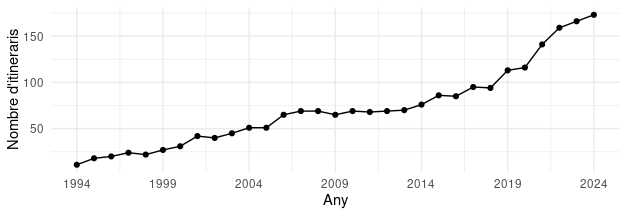
\includegraphics[width=0.8\textwidth]{No_of_itineraris_per_any.png} % Ajusta el ancho de la imagen
    \caption{Evolucio del nombre d'itineraris de la xarxa CBMS al llarg del temps actiu.} % Título de la imagen
    \label{fig:mi_imagen} % Etiqueta para referenciar la imagen en el texto
\end{figure}

 \begin{figure}[h!] % [h!] es una sugerencia de posicionamiento (aquí)
    \centering % Centra la imagen
    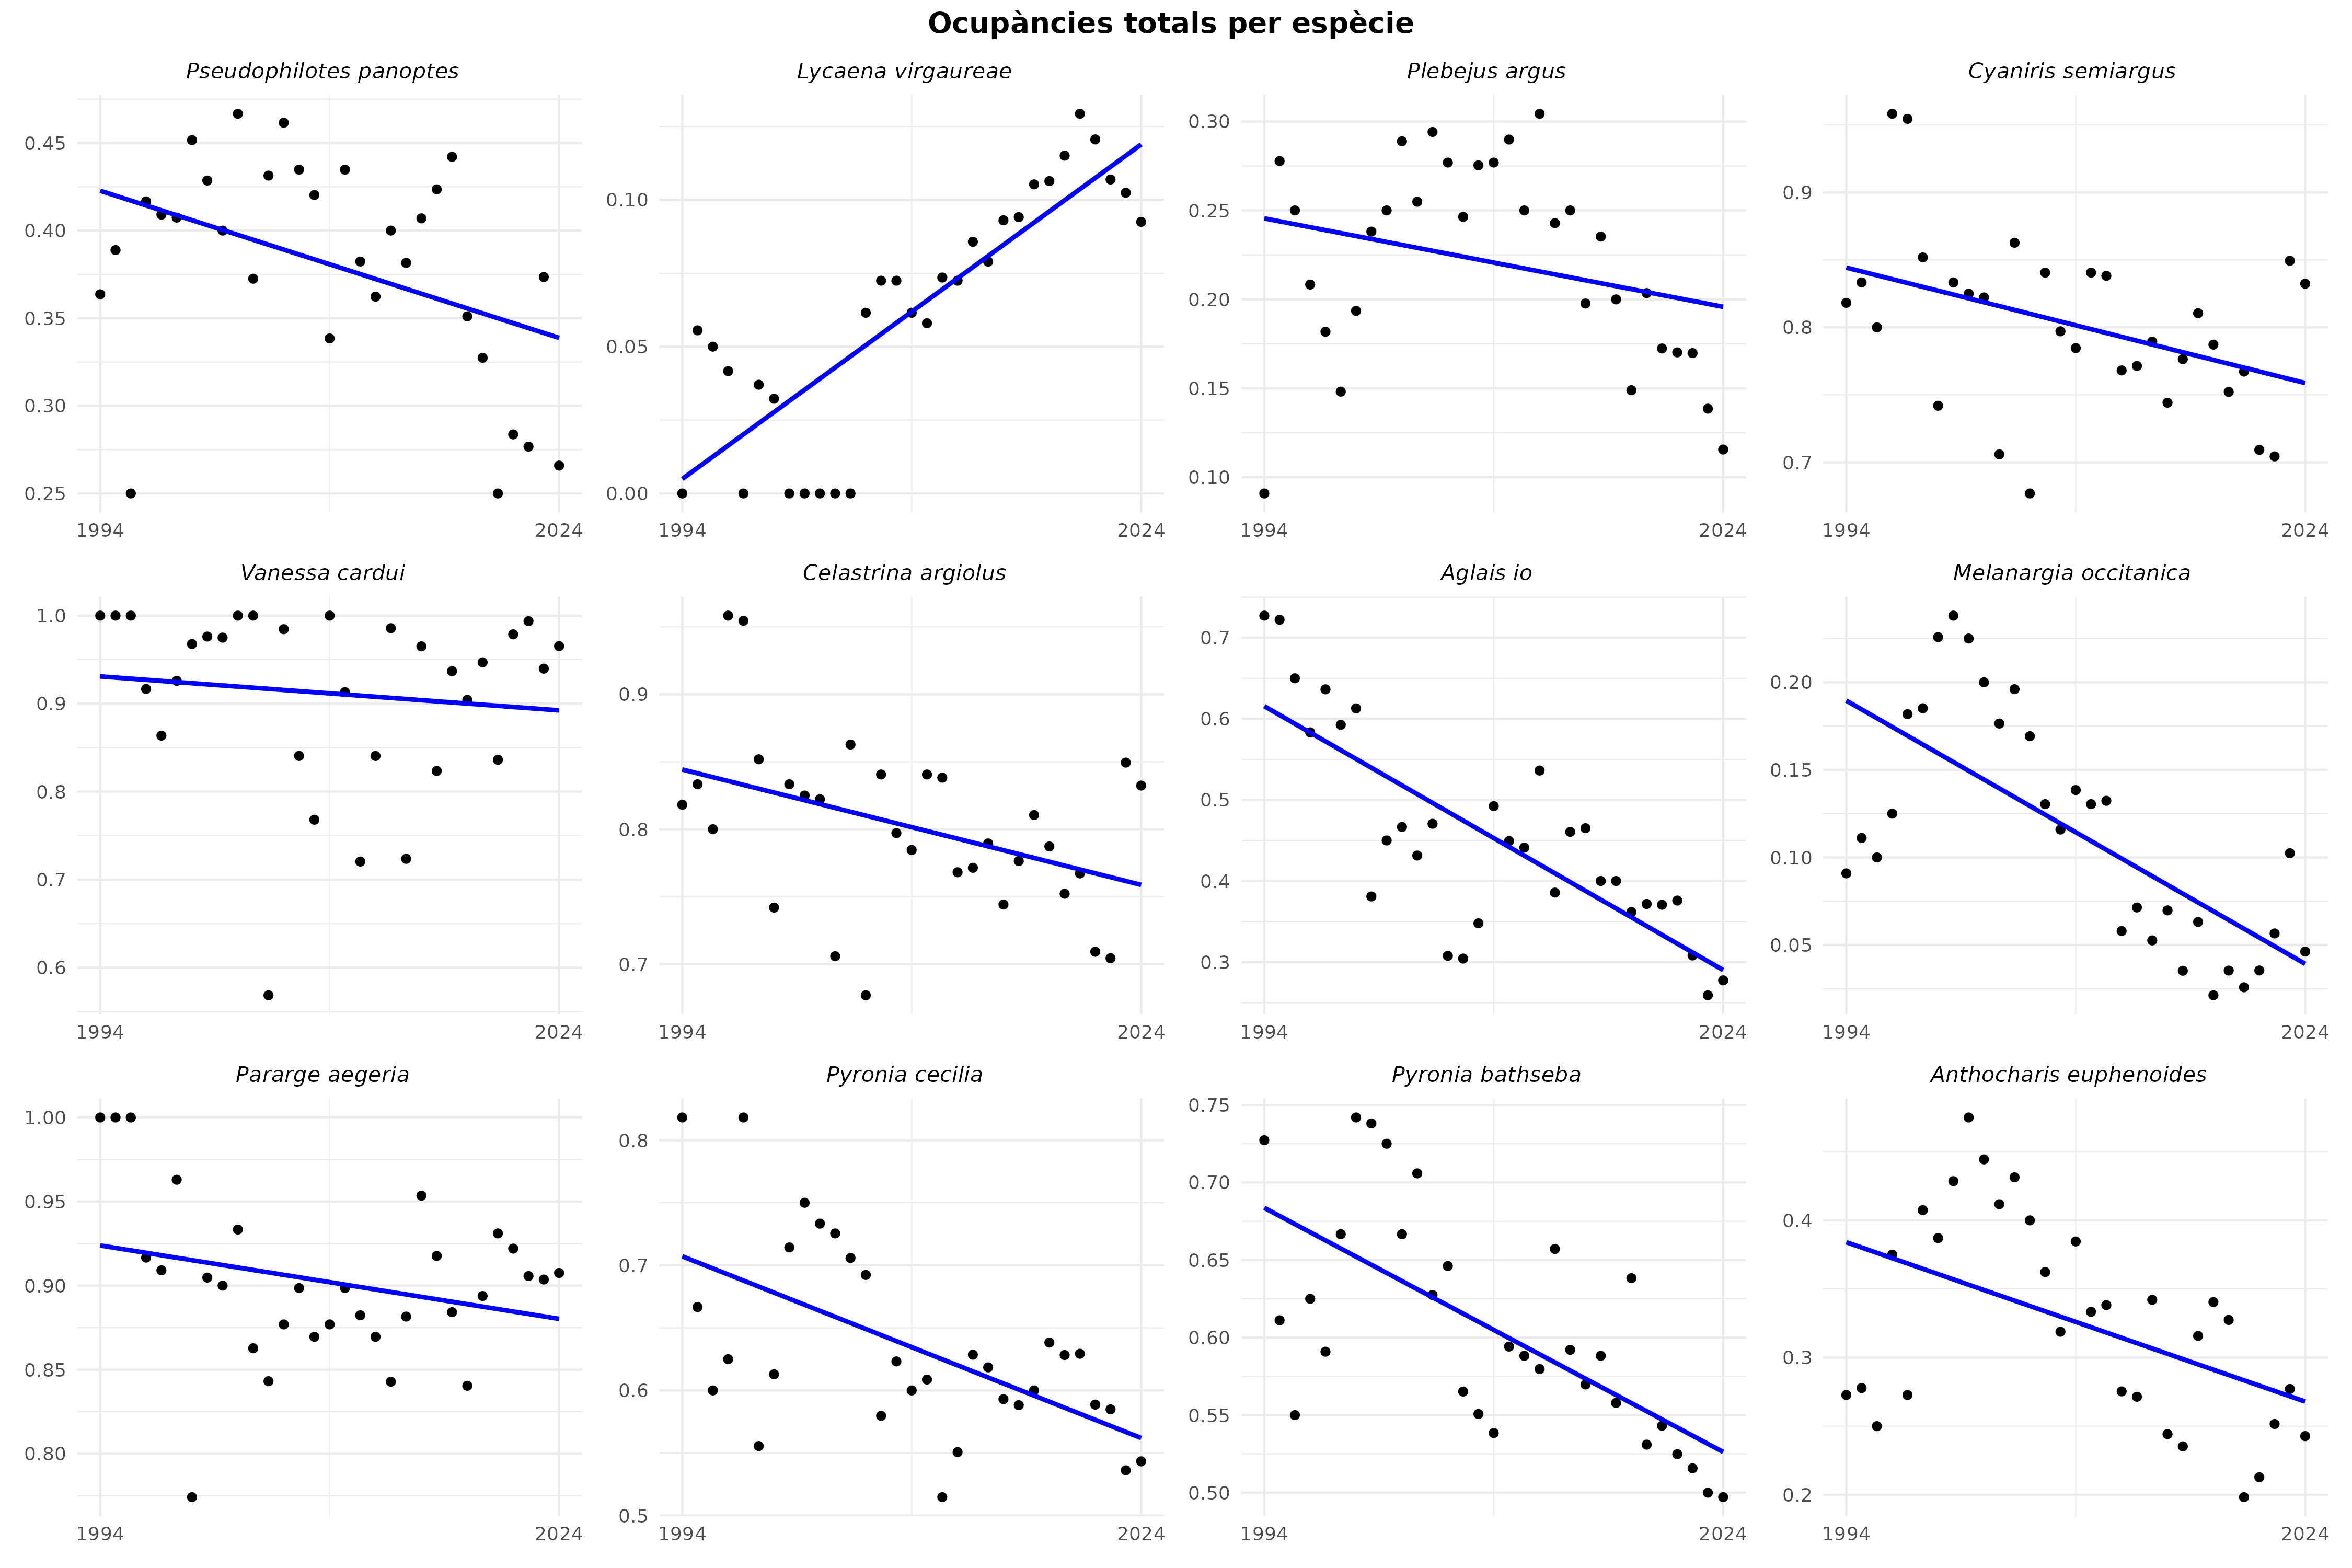
\includegraphics[width=0.8\textwidth]{ocupancies_totals.png} % Ajusta el ancho de la imagen
    \caption{Ocupancia de les especies en tots els itineraris} % Título de la imagen
    \label{fig:mi_imagen} % Etiqueta para referenciar la imagen en el texto
\end{figure}



    \item Representar les taxes annulas de $c$ i $e$ de les 12 esp\`ecies en un "scatter plot". 

     \begin{figure}[h!] % [h!] es una sugerencia de posicionamiento (aquí)
    \centering % Centra la imagen
    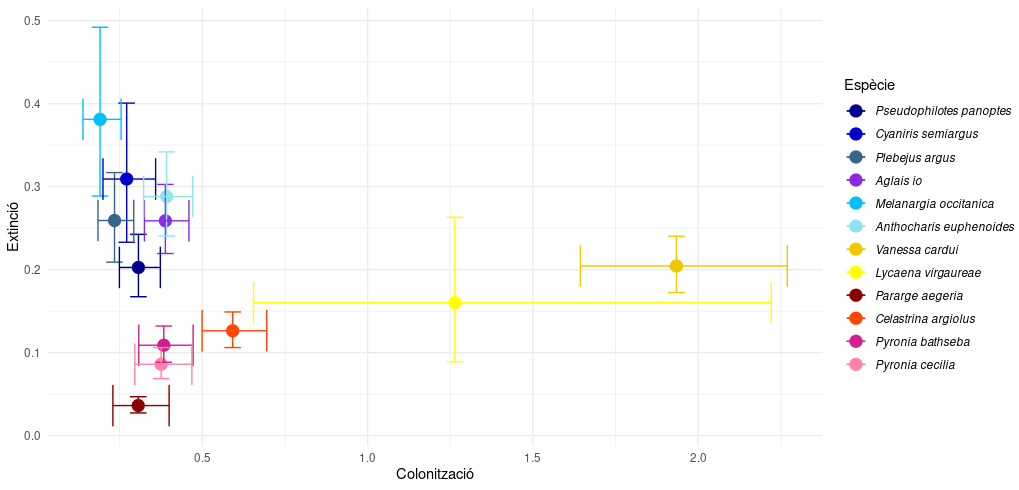
\includegraphics[width=0.8\textwidth]{colext_total.png} % Ajusta el ancho de la imagen
    \caption{Valors de colonitzacio i extincio amb les barres d'error de cada especie calculats amb les dades des de l'any 1994 fins el 2024. } % Título de la imagen
    \label{fig:mi_imagen} % Etiqueta para referenciar la imagen en el texto
\end{figure}

    \item Fer un arbre dicot\`omic amb els valor de colonitzacio i extenci\'o de les esp\`ecies i utilitzar selecci\'o de models (AKAIKE) per a determinar l'agrupaci\'o m\'es parsimoniosa. 
    
    \item Assignar barres d'error a aquestes estimes, $(c, e)$, de m\`axima versemblan\c{c}a.
    
    \item Interpretar la NLL per transici\'o com una mesura de "goodness-of-fit" que ens permeti comparar entre ajustos i hip\`otesis. 
    
    \item Estudiar si els par\`ametres de $c$ i $e$ es correlacionen amb els indexos de SSI, HPI i mobilitat.  
    
    \item Estudiar si la caracteritzaci\'o de cada esp\`ecie en termes del parell de par\`ametres $(c, e)$ depen de la zona bioclim\`atica. Fer selecci\'o de models segons el criteri d'AKAIKE. 
    
    \item Estudiar si la caracteritzaci\'o de cada esp\`ecie en termes del parell de par\`ametres $(c, e)$ depen de l'al\c{c}ada respecte el nivell del mar. Cal calcular la colonitzaci\'o i extinci\'o de cada esp\`ecie en cada intinerari. Cal descartar aquells c\`alculs on hi hagi molt poques transcions, \'es a dir, on les barres d'error dels par\`ametres siguin massa grans.'
    
    \item Anova d'un factor (regi\'o bioclim\`atica) que est\`a classificat en tres nivells (alpina-subalpina, mediterr\`ania humida i medeterr\`ania \`arida) de la colonitzacio (i per separat de l'extinci\'o) de cada especies en cada itinerari. 
\end{enumerate}

Hem fet el Mantel test entre la matriu de dist\`ancies geogr\`afiques entre itinierais i la matriu de dist\`ancies ecol\`ogiques, on cada itinerari estaria representat per un punt en el pla colonitzaci\'o - extinci\'o. Aquest ha estat el resultat: Mantel statistic r: 0.009039 (Significance: 0.413). Si itineraris allunyats entre si tinguessin din\`amiques de colonitzaci\'o-extinci\'o molt differents, seria esperable que la correlaci\'o entre dist\`ancies geogr\`afiques i ecol\`ogiques result\'es positiva, per\`o, en aquesta an\`alisi, ens surt baix\'issima (0.009039). A m\'es, el p-valor (Significance) ens diu que aquesta correlaci\'o no \'es gens significativa.     

\newpage

\section{Conclusions}
\subsection{Perspectives futures}


\newpage
\printbibliography

\end{document}



